\label{sec:intro}

\subsection{Motivation}
High-quality web applications need to provide both good functionality 
--- informative and well-displayed web-page content, 
and good performance --- lower than 2 seconds of page load
time \cite{nah2004study}, with every second's delay causing 11\% fewer page views, a 16\% decrease in customer satisfaction, and 7\% loss in conversions~\cite{onesecond}. 
These functionality and performance requirements are 
increasingly difficult to satisfy {\it simultaneously}, as modern web-page content
often requires processing a huge amount of 
user data to generate and the amount of user data often increases by 10$\times$ per year \cite{startup}. 
Indeed, real-world web developers often don't understand the amount of data processing required to render their web pages, which results in numerous design changes to address performance issues~\cite{yang:icse18:hloop}.
%certain web-page element and have to change their web-page designs 
%to solve performance complaints from web users~\cite{yang:icse18:hloop}.
Because of this, tools that can help developers understand
performance implications of their web-page design and explore designs
with different performance-functionality trade-offs can greatly improve the web development process.


\iffalse
Even worse, web applications are often highly modularized,
with data maintenance (model), web-page displays (view), and control logic
(controller) separately designed and implemented, making holistic performance 
understanding and optimization difficult. \cong{Isn't it just inter-procedure analysis? Why is it difficult?}
\fi



%\cong{How about discussing 1. slow webpages are bad (as above); 2. mention old work on semantic-preserving changes, and say that they are usually not enough; 3. non-semantic preserving changes requires functionality-performance tradeoff, give examples of less features on webpages for better performance; 4. developers do not know well about how to make such tradeoff, mixed language and programming model (html/javascript/ruby, object-oriented/relational) makes it hard to understand the time breakdown. Currently tools can analyze performance for only one of the language or only client side. But to make such tradeoff, developers need a holistic view of what contributes to each webpage functionality, database, server or client. (I make a skeleton in the comment below)}

%... 10x per year. \cong{say more about current webpages are slow. maybe cite some complains from issue reports?}
%
%Previous work has done on improving the performance of these web applications. For example, \cite{powerstation} identifies inefficient API usage and replace with better API, ..., \cite{chen.tse} ...., etc. These tools apply semantic-preserving changes to application source code and bring substantial performance improvement. However, the study \cite{yang.icse18} shows that non-semantic-preserving changes like pagination and removing webpage features bring much larger performance gain. Semantic-preserving optimizations achieve 2.16$\times$ average speedup (up to xx$\times$), while non-semantic-preserving ones achieve 8.79$\times$ average speedup (up to xx$\times$). For many pages, it is even impossible to accelerate without modifying the page content.

%Indeed, it is often seen in issue reports that developers sacrifice functionality for better performance. For instance, ... \cong{show the tracks example here}.

%Unfortunately, it is not trivial to make such functionality-performance tradeoff. To debug a slow webpage and remove expensive features as described above, a developer need to trace how each webpage component is generated. To render the toolbar, the application first issues a SQL query to ... using Rails API as .... Then it ... \cong{describe the process, emphasize on the different language involved.} Furthermore, to understand the cost, a developer needs to know how expensive the query is, \cong{anything more?}. Existing tools...

%Even worse, these applications are structured in a very modularized way. Most web-applications adopt MVC architecture.\cong{If you think MVC is a problem, discuss it here.} 

%As we can see, to make functionality-performance tradeoff, developers need to have a holistic view of what contributes to each webpage feature, from queries issued to the database, how returned tuples are processed, to how data are rendered on the client side. It becomes even harder when no test database is available. Without large-enough test data, ...



% \iffalse
% A web application often involves a client side running
% in the browser, an application server running the control logic,
% and a back-end database management system (DBMS) hosting persistent user data, reflecting
% the widely used model-view-controller (MVC) software architecture.
% \alvin{why is this paragraph here? last paragraph already mentions MVC?}

% Bridging the controller and the model, 
% object-relational mapping (ORM) framework, such as Ruby on Rails \cite{ruby}, 
% Django \cite{django}, and Hibernate \cite{hibernate}, is widely used to map 
% persistent data stored in DBMS to heap objects and to transparently translate
% object-oriented code written by web developers into SQL queries at run time. 
% \alvin{Is this point of the previous 2 paragraphs to explain how web apps are structured? If so I'd explain it that way. Right now it feels like a random collection of paragraphs}

% Bridging the view and the controller, embedded templating systems, 
% such as eRuby and Haml,  can mix content dynamically generated by controller
% with static HTML templates, and enable developers to easily specify which controller
% variables should be rendered inside which HTML tag. \alvin{why mention this?}

% Unfortunately, although improving productivity, this programming paradigm
% brings challenges in understanding and optimizing functionality--performance
% tradeoffs \alvin{what does this mean?} in web development. With ORM, developers writing controller code 
% cannot easily know what database queries will be issued at run time and how expensive their code actually is. With embedded templating systems, 
% developers doing view design cannot easily know the generation-cost
% or the generated amount of data rendered in an HTML element.
% Consequently, they cannot easily decide which data should be displayed
% and in which style. \alvin{so are we saying that MVC and ORM are both bad and should be abolished?}
% %are time-consuming but unworthy, because it is hard to estimate the performance cost of a new feature, given that ORM abstracts what queries will be issued, how queries will be executed, and how much data will be returned from the DBMS behind a new feature. 
% \fi



To better understand the challenges faced by web developers, consider
Tracks~\cite{tracks}, a popular 
task-management application constructed using the Ruby on Rails framework. 
Tracks has a {\tt todos/index} page displaying all the to-do's
for a user. At one point, users complained that
this page was unreasonably slow even though very few to-do's were displayed \cite{tracks870}. 
After some debugging, developers turned their attention to a sidebar on this page, which displayed all the projects the user had been involved in. As shown in 
Figure \ref{fig:crossstack},
the view file {\tt sidebar.html.erb}, which produces this sidebar, renders these projects based on a Ruby variable 
{\tt @active\_projects} embedded in the HTML file; this variable is computed in 
a controller Ruby file {\tt todos\_controller.rb} through a seemingly straightforward 
assignment {\tt @active\_projects = user.projects.active}. It turns out that this code actually retrieves objects stored in a database, and is 
translated into a SQL query by the Rails
framework at run time. It was the long time taken for the database to run this query that resulted in the poor performance observed by users. 
%\cong{We haven't introduced what is a 'view file' or the ORM structure, so mentioning ``view file'' and the controller process seems a bit redundant. suggestion: either move this example to after we introduce the challenges, or not mention all the details and say sth like ``a sidebar is expensive to compute, and developers find it is due to a slow query that cannot be accelerated.''}
%\shan{Cong, I get your concern. How about I simply delete
%``Object Relational Mapping'', and just say "xx was translated into a database query at
%run time''? I don't want to 
%delete all the details, because that would lose the point of being an example.}
%\cong{Yes I agree with keeping the details. I'm just afraid we haven't introduced ORM and MVC, so the ``view file'' and ``controller file'' may be a bit confusing? Or we may simply mention MVC architecture and say ``view module''. And also we can emphasize that in the {.erb} file the ruby variable {\tt @active\_projects} is embedded within HTML, as people who don't know {.erb} file may not be aware of that.}
%\shan{Make sense. I will do another pass of this paragraph}
After realizing this, developers decided to remove the sidebar \alvin{remove what?}, and 
users can now see the main content of this page, the to-do items, much quicker.


% A recent study on 12 popular applications shows that a lot of performance problems can be solved by changing the application design such as adjusting application display or removing costly functionalities, which also achieves large performance improvement. 

% Unlike other performance problems caused by API misuse or database design, 
%requires not only the back-end profiling, but also the front-end display. 
\begin{figure}
 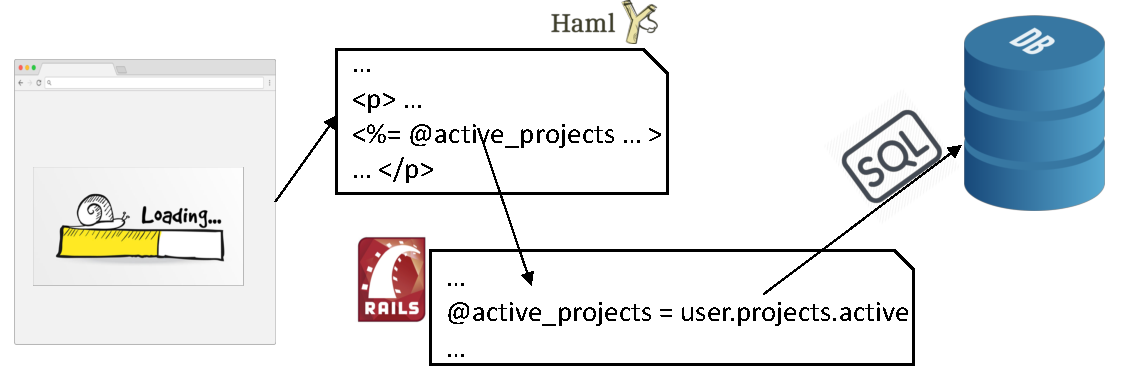
\includegraphics[width=\columnwidth]{figs/crossstack.pdf}
\vspace{0.1in}
\caption{Performance understanding challenge}
\label{fig:crossstack}
\vspace{-0.2in}
\end{figure}

This performance-functionality trade-off represents one of the many challenges that web developers face:

{\bf Understanding the performance cost} behind every rendered web-page element is challenging for developers and requires cross-stack knowledge as the above example shows.
As shown in Figure~\ref{fig:crossstack}, modern web pages commonly contain
dynamically generated contents. Consequently, the cost of a web-page element
includes not only browser rendering time, but also web server
computation time and backend database server processing time.
As web applications are often constructed using 
the Model, View, Controller~\cite{mvc} architecture, 
it is difficult for users to manually search through multiple files 
across application modules to identify code that leads to performance issues, and it is even more difficult for developers
to reason about what database queries could be issued as their application executes and how much data would be retrieved from database for rendering.

% \iffalse
% To help developers get a holistic {\textit understanding} of web-application performance, a tool should ideally
% (1) be view-centric, enabling developers to understand the cost behind every HTML tag
% and make fine-granularity performance-aware web-design decisions. 
% (2) be aware of the underlying database, accounting for not (only) the client-side rendering cost, 
% but (also) the database query processing time, which is often very expensive and difficult for 
% developers to manually figure out; \alvin{why are `only' and `also' in parens?} \cong{cross-stack or cross-language rather than just ``aware of database''} (3) work with or without sufficient testing workload. \alvin{don't get what (3) means}
% It is challenging to synthesize large database workload \cite{xxx} \alvin{why? because it needs to be realistic?}. If the tool solely relies on 
% dynamic profiling, many performance bottlenecks would escape in-house testing.
% \fi

Existing profiling tools are insufficient in aiding with this regard.
Some~\cite{chromeDev} only account for the client-side
cost of every HTML tag, but do not account for the server-side cost;
others~\cite{arqt} report database query cost but do not attribute
queries to specific HTML tag, and hence cannot provide direct guidance to
web-page design. Furthermore, all these profiling tools rely on 
workloads provided by developers, and therefore cannot help predict
performance problems that manifest from ``real-world'' workloads.
%future workload unavailable at in-house testing.

%However, the previous work can barely assist developers in better application design because developers need more information about the performance cost behind a new feature and should be  provided with various alternative design choices like pagination with better performance.  This support hasn't bee provided yet due to the following challenges:
%it is important to give them deeper understanding of the performance implication of their design. 

%loop complexity~\cite{suzuki1996efficient}, however, the 
%traditional cost model no longer works for ORM frameworks due to its cross-stack architecture. 

%Secondly, the existing  dynamic profiling tools can only find out the performance cost either on a single query or a view file, neither can completely reflect the performance cost of a new feature of the complicated nature of the feature. There doesn't exist an one-to-one mapping relation between a new feature and a query or a view file. 

%Thirdly, the performance cost under dynamic profiling also has a lot to do with the workload. There is no way that we can estimate  the possible performance cost for all workloads through profiling.


{\bf Exploring the performance-functionality trade-offs} among different web-page
designs is also challenging for developers, requiring cross-module and cross-language
code refactoring. For example, to remove a web-page element, it is insufficient
to just remove the corresponding HTML tag from the view file. 
Developers also need to check which variables are referred to by that HTML tag, which controller code snippets generated those variables, and whether removing those code snippets altogether will affect other parts of the application. In addition, there are also other web-page design alternatives
with different performance-functionality tradeoffs. Unfortunately, most require global code restructuring and are difficult to carry out without tool support.
%
%Existing code refactoring and compiler optimization cannot help, as the task here involves changes to software functionality (i.e., web-page design).
Worse yet, recent work on detecting and fixing database-related inefficiencies in
web applications only focuses on
inefficient ORM-API usage, unnecessary data retrieval, and redundant queries~\cite{mark:icse16:javascript, chen:se16:redundantData, yang:fse18:powerstation},
and is completely oblivious to web-page designs. In short, existing
techniques do not consider performance-enhancing opportunities that require 
web-page design changes (which we refer to as {\it view changes}), and hence
cannot help developers explore the performance-functionality trade-off space.
%, and
%also cannot provide optimization suggestions towards performance-bottlenecks associated with
%specific view components.

Indeed, empirical studies~\cite{yang:icse18:hloop} have found that about a quarter of real-world web application performance problems are solved by
developers through view changes, like pagination and view content removal.
These changes often bring much more performance improvement
than the view-preserving ones (8.79$\times$ vs 2.16$\times$ on average) but involve more changes (2.9 files vs. 1.4 files). They are difficult to perform manually and having good tooling support is hence crucial.



%of model, view, and controller. Previous work xxx
%There exists some work aims to solve specific performance problems of web applications built upon ORM framework. Some has identified the unnecessary data retrieval in applications built using both Hibernate~\cite{chen:se16:redundantData} and
%Rails~\cite{cong.cikm17}; some targets on the N + 1 query~\cite{chen:se14:antipattern}; some improves the performance by pushing down the computation to DBMS~\cite{pldi13}; and some automatically batches queries.  
%Finally, it's also non-trivial to decide alternative design choices and how to change their code correctly because one feature could involve multiple files and one change could affect multiple features.

%Also However, this kind of support has not been provided yet.

\subsection{Contributions}
In this work, we present a framework called \Tool that provides a view-centric 
and database-aware analysis
for web developers to understand and optimize 
their database-backed web applications. \Tool currently targets applications  written using the Ruby on Rails framework, and makes three major contributions as illustrated in Figure \ref{fig:overview}.

\Tool provides a view-centric estimator that helps developers understand the 
data-processing cost behind every HTML tag. 
\Tool both dynamically monitors database query performance using the test workload, statically estimates data processing complexity independent of any specific workload, and carefully attributes the cost to every HTML tag
through its cross-stack dependency analysis. The details will be presented in 
Section \ref{sec:profile}.

\Tool provides a view-aware performance optimizer that helps developers carry out
view-changing code refactoring to improve performance. \Tool suggests a variety
of refactorings that (1) change the manner of content rendering (i.e., pagination or asynchronous loading);
or (2) change the accuracy of the rendered contents (i.e., approximation);
or (3) remove certain web-page contents from rendered contents. Through static program
analysis, \Tool not only identifies opportunities for applying such refactoring,
but also automatically suggests patches that complete such refactoring,
often involving modifications to multiple files in model, view, and controller components.
We present the details in Section \ref{sec:opt}.

%We estimates the performance cost for each HTML tag that will be rendered on the page through dynamic run-time logging and static analysis, which is a new granularity for performance estimation. Also our approach includes the wall-clock performance cost and relative performance cost towards the database size. As a result, this approach also works when there is not a representative workload for us to gain enough performance cost information. 

\Tool provides a unique interface for developers to effectively
exploring different web-page designs with different performance-functionality trade-offs.
Instead of separately presenting profiling information and refactoring suggestions, \Tool integrates them in the web browser---while testing a page of their web applications, the data processing cost for each HTML tag is presented as a heat map in the browser. Developers can right click on each
HTML tag to see the different view-changing options for performance enhancement; they can 
choose any option and immediately see an updated web page with an updated heat map in the browser,
with all code refactoring automatically done by \Tool in an accompanying Ruby editor.
%Section \ref{sec:im} explains how \Tool implements this interface through a combination of
%Ruby editor plug-ins, \Tool performance-debugging JavaScript, and static instrumentation 
%of the web application under development.

%Users can easily explore various types of optimizations 
%before they decide on the most suitable design that gives the 
%best balance between web-page functionality and page-loading performance. 
%\alvin{this paragraph seems to be more of a description of how \Tool works. I suggest moving this somewhere else and state precisely what is new about the \Tool interface here instead}

%Secondly, we implement this approach into a prototype on Ruby on Rails framework through Rails libraries and RubyMine IDE plugin. 




\begin{figure}
    \centering
    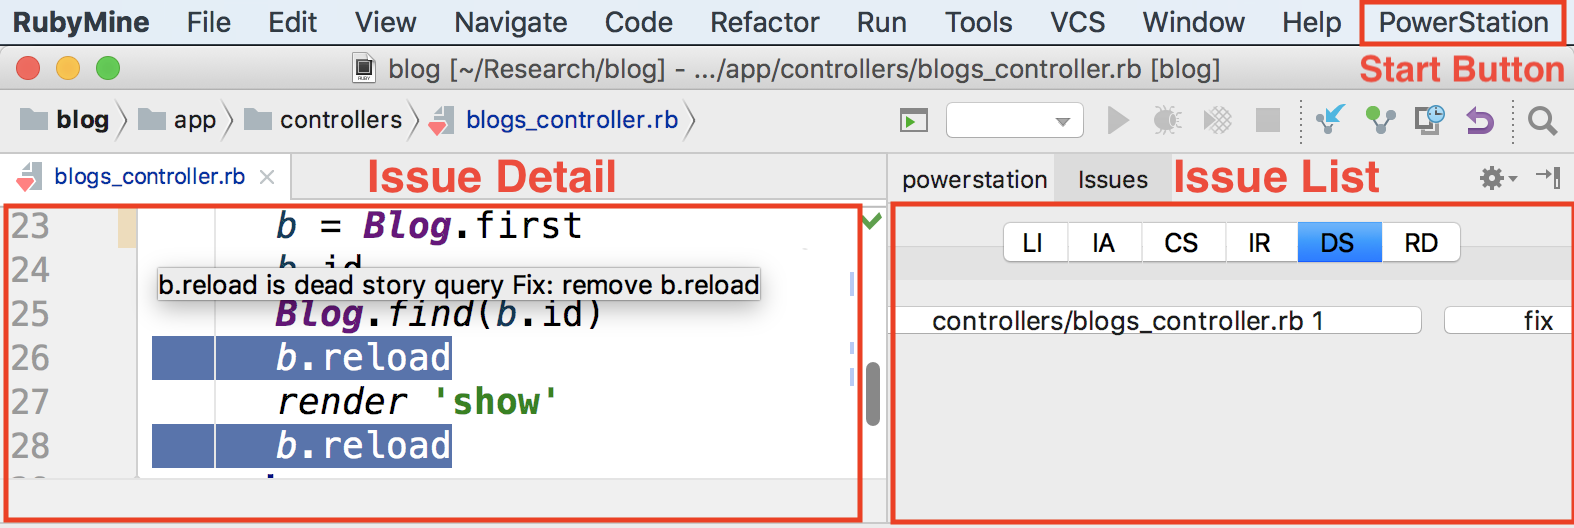
\includegraphics[width=\columnwidth]{figs/overview.pdf}
    \vspace{-0.1in}
    \caption{\Tool overview}
     \vspace{-0.2in}
    \label{fig:overview}
\end{figure}


We evaluated \Tool on 12 popular open-source Ruby on Rails applications.
\Tool statically identifies \numissues performance-enhancing
opportunities through view changes. We randomly sampled 15 view changes suggested
by \Tool and found that by applying the patches automatically generated by \Tool,
these 15 view changes speed up end-to-end page load time by \eoespeedup on average
(\maxspeedup maximum), using database workloads that are similar to those used in real-world deployments. We believe the benefits will increase with even larger workloads. %a larger workload will offer even bigger speedup.
Furthermore, we conducted a thorough user study with 100 participants from
Amazon Mechanical Turk. The study shows that web pages with these
view changes are considered as similar or better than the original web pages
in most cases, with more users preferring the design suggested by
\Tool than the original ones. This user study result, as well as the fact 
that these optimizations save computation resources on web servers and database servers, justify the need for developers to explore the performance-functionality 
trade-off space in web application design, with \Tool being a first step towards that goal.